\begin{exercice}
Dans chaque cas, précise si les droites $(d_1)$ et $(d_2)$ sont ou non parallèles et pourquoi.

\begin{center}
    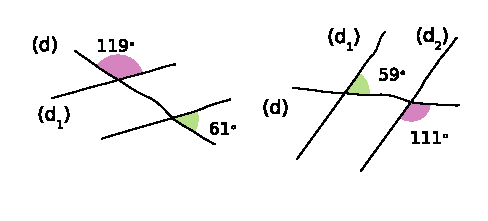
\includegraphics[width=\linewidth]{exoApp1}
\end{center}

\end{exercice}



\begin{exercice}[Triangle isocèle]

\begin{center}
    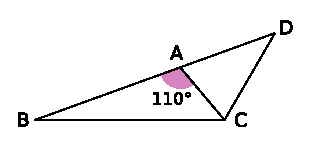
\includegraphics[width=.8\linewidth]{exoApp2}
\end{center}

La figure ci-dessus est telle que :
\begin{itemize}
    \item $B$, $A$ et $D$ sont des points alignés ;
    \item $\widehat{BAC}$ et $\widehat{ACD}$ sont supplémentaires ;
    \item $\widehat{BAC}$= 110°.
\end{itemize}

\begin{enumerate}
\item Montre, en justifiant, que les angles $\widehat{DAC}$ et $\widehat{ACD}$ sont égaux à 70°.
\item Montre alors que le triangle $ADC$ est isocèle.
\item De plus, l'angle $\widehat{ACB}$ mesure 50°. Montre, en justifiant, que les angles $\widehat{BCA}$ et $\widehat{ADC}$ sont complémentaires.
\item Trouve, en justifiant, deux autres paires d'angles complémentaires.
\end{enumerate}
\end{exercice}




\begin{exercice}[Parallèles ou non ?]

\begin{center}
    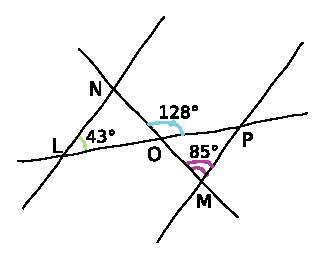
\includegraphics[width=.8\linewidth]{exoApp3}
\end{center}

La figure ci-dessus est tracée à main levée.

\begin{enumerate}
\item Calcule la mesure de l'angle $\widehat{LON}$.
\item Déduis-en la mesure de l'angle $\widehat{ONL}$.
\item Détermine alors si les droites $(LN)$ et $(MP)$ sont parallèles.
\item Sachant que les segments $[LN]$ et $[MP]$ sont de même longueur, détermine la nature du quadrilatère $LNPM$.
\end{enumerate}
\end{exercice}




\begin{exercice}[Un isocèle de plus]

\begin{center}
    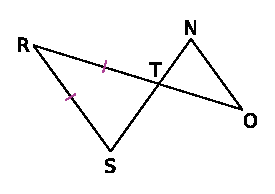
\includegraphics[width=.6\linewidth]{exoApp4}
\end{center}

La figure ci-dessus est telle que :
\begin{itemize}
    \item les droites $(RO)$ et $(SN)$ sont sécantes en $T$ ;
    \item le triangle $RST$ est isocèle en $R$ ;
    \item les droites $(RS)$ et $(NO)$ sont parallèles.
\end{itemize}

Montre que le triangle $TNO$ est isocèle.
\end{exercice}




\begin{exercice}[Un périscope de fortune !]

\begin{enumerate}
\item Fais une recherche sur Internet concernant la loi de réflexion de la lumière.
\item Le schéma ci-dessous illustre un rayon de lumière qui se réfléchit sur un miroir avec un angle de 30°. Détermine $\hat{x}$ et $\hat{y}$. Justifie.

\begin{center}
    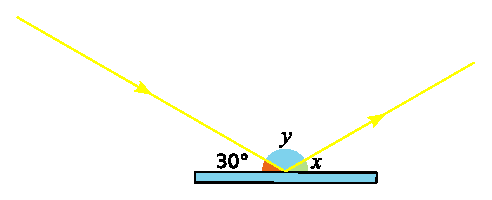
\includegraphics[width=.8\linewidth]{exoApp5}
\end{center}

\item Éric a construit un périscope avec une boîte de carton et deux miroirs parallèles comme l'illustre le schéma ci-dessous.

\begin{center}
    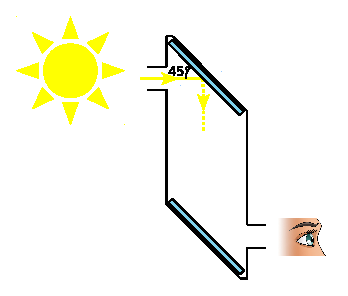
\includegraphics[width=.8\linewidth]{exoApp6}
\end{center}

\begin{itemize}
    \item Si un rayon entre horizontalement dans le périscope, en sortira-t-il horizontalement aussi ?
    
    (Tu pourras montrer que les rayons d'entrée et de sortie sont parallèles.)
    \item Ce résultat dépend-il de l'inclinaison des miroirs parallèles ?
    
    (Autrement dit, a-t-on le même résultat si l'angle formé par le rayon et le miroir est différent de 45° ?)
\end{itemize}
\end{enumerate}
\end{exercice}
